\documentclass{article}

\usepackage{ocencfd}
\usepackage{geometry}
\usepackage{graphicx}
\usepackage{float}
\usepackage{amsfonts}
\usepackage{mathrsfs}
\usepackage{mwe}
\usepackage{subfig}

\title{Introduction to Deep Learning\\Assignment 2} % Sets article title
\author{\textbf{Group 53}\\Chenyu Shi (s3500063); Shupei Li (s3430863); Shuang Fan (s3505847)} % Sets authors name
\documentID{Introduction to Deep Learning Assignment 2} %Should be alphanumeric identifier
\fileInclude{} %Names of file to attach
\date{\today} % Sets date for publication as date compiled
\graphicspath{{fig/}}
\geometry{a4paper, left=2cm, right=2cm, top=2cm, bottom=2cm}

% The preamble ends with the command \begin{document}
\begin{document} % All begin commands must be paired with an end command somewhere

\maketitle % creates title using information in preamble (title, author, date)

\section*{Task 1}
\setcounter{section}{1}
\setcounter{subsection}{0}
\subsection{Official Repository Examples}
We reproduce the results of \texttt{mnist\_mlp.py} and \texttt{mnist\_cnn.py} for the MNIST dataset. Without adjusting model architectures, Table \ref{tab:1-offer} reports our experimental results.
\begin{table}[!ht]
    \centering
    \caption{MNIST: Official Repository Examples}
    \label{tab:1-offer}
    \begin{tabular}{llllll}
        \toprule
        \textbf{Model} & \textbf{\#Epoch} & \textbf{Test Loss} & \textbf{Test Accuracy}\\
        \midrule
        MLP & 20 & 0.1206 & 0.9837\\
        CNN & 12 & 0.4189 & 0.8891\\
        \bottomrule
    \end{tabular}
\end{table}

\subsection{Exploratory Experiments}
Based on the experience we learned from Keras official documentation, we set the model architectures provided in the textbook as benchmarks and try different hyperparameter settings on Fashion MNIST and CIFAR-10 datasets. It is worth noting that we set the number of epoches to 50 and use early stopping technique during the hyperparameter tuning process. We also add model checkpoints to save the weights of the best model and load the weights when evaluating the performance. The combination of early stopping and model checkpoints dynamically balances between training costs and model performance. The following describes our experiments in detail.

\subsubsection{Fashion MNIST}
\textbf{MLP}. Firstly, we adjust the number of layers as well as hidden layer units to determine the best model architecture. Table \ref{tab:1-ma-mnist} summarizes the results of different model settings. And Figure \ref{fig:1-mlp-arch} illustrates the changing trends of validation accuracy during the training.
\begin{table}[!ht]
    \centering
    \caption{MLP Model Architectures}
    \label{tab:1-ma-mnist}
    \begin{tabular}{llll}
        \toprule
        \textbf{Parameter} & \textbf{Value} & \textbf{Test Loss} & \textbf{Test Accuracy}\\
        \midrule
        \#layers & 2 & 0.3679 & \textbf{0.8911}\\
                 & 3 & 0.3622 & 0.8843\\
                 & 4 & 0.3583 & 0.8842\\
        \midrule
        \#units & 128 & 0.3659 & \textbf{0.8876}\\
                & 256 & 0.3302 & 0.8847\\
                & 512 & 0.3539 & 0.8858\\
        \midrule
        Baseline & - & 0.6186 & 0.8863\\
        \bottomrule
    \end{tabular}
\end{table}
\begin{figure}[!ht]
    \centering
    \subfloat[\#layers]{%
        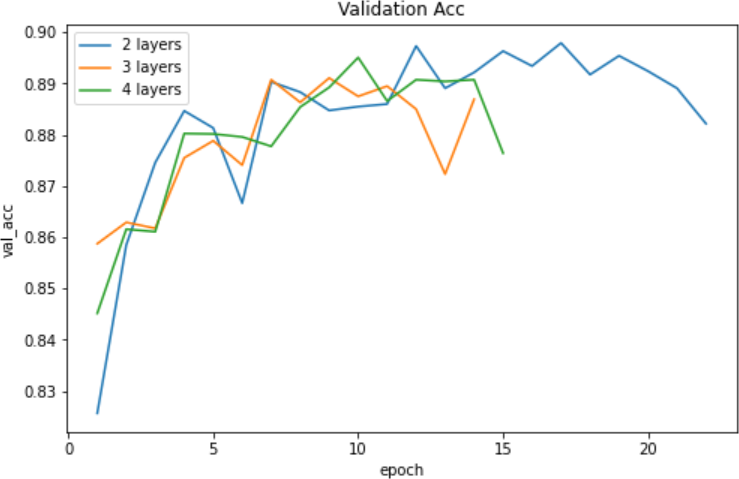
\includegraphics[width=6cm]{./fig/1-layer.png}%
        }%
        \hspace{1cm}
    \subfloat[\#units]{%
        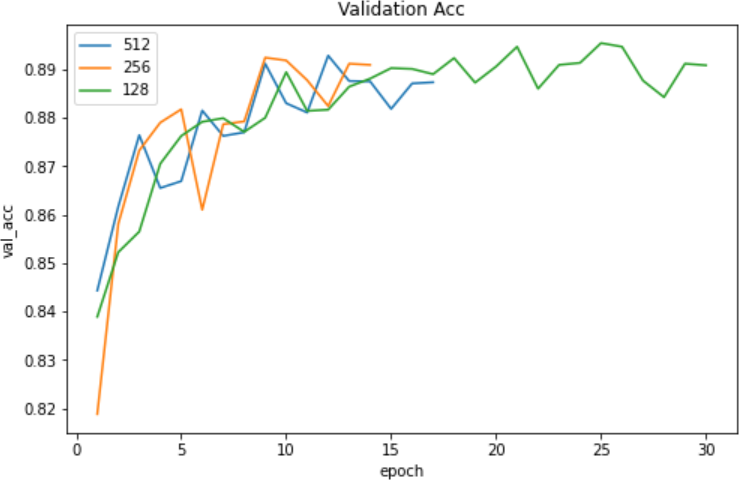
\includegraphics[width=6cm]{./fig/1-unit.png}%
        }%
    \caption{MLP: Validation Accuracy}
    \label{fig:1-mlp-arch}
\end{figure}
\par
According to the results,  MLP model with two layers and 128 units is the best model. Therefore, we adopt this architecture when exploring other hyperparameters. We follow the hints in the assignment description and experiment with initializations, activations, optimizers, and regulariztions. Table \ref{tab:1-hy-mnist} summarizes the options we have tested.
\begin{table}[!ht]
    \centering
    \caption{MLP Hyperparameter Tuning}
    \label{tab:1-hy-mnist}
    \begin{tabular}{lll}
        \toprule
        \textbf{Category} & \textbf{Parameter} & \textbf{Values}\\
        \midrule
        Initialization & kernel initializer & RandomNormal, GlorotNormal, GlorotUniform\\
        Activation & layer activation & relu, sigmoid, tanh\\
        Optimizer & optimizer & RMSprop, Adam (learning_rate=0.001), Adam (learning_rate=0.01)\\
        Regularization & kernel regularizer & None, L1, L2\\
                       & Dropout layer & With / Without one dropout layer after the hidden layer.\\
                       & dropout rate & 0.1, 0.3, 0.5 (The dropout rate when adding the Dropout layers)\\
        \bottomrule
    \end{tabular}
\end{table}
\par
We begin with models without Dropout layers, considering the relatively large parameter space. Grid search method is used to optimize hyperparameters, which leads to 81 different settings. The detailed results can be found in the jupyter notebook. And we omit results here due to the limited space. The best model without dropout layers has the setting: \{kernel initializer: GlorotUniform, layer activation: sigmoid, optimizer: RMSprop, kernel regularizer: None\}. Based on that, we add dropout layers to the model with different dropout rates. Table \ref{tab:1-top3-mlp} lists the top three MLP model settings. The layer activation, kernel initializer, and optimizer of these settings are relu, GlorotUniform, RMSprop respectively. All settings don't use the kernel regularizer.
\begin{table}[!ht]
    \centering
    \caption{Top Three MLP Model Settings}
    \label{tab:1-top3-mlp}
    \begin{tabular}{lllll}
        \toprule
        \textbf{Model} & \textbf{\#layers} & \textbf{\#units} & \textbf{Dropout Layer} & \textbf{Test Accuracy}\\
        \midrule
        Top 1 & 2 & (512, 10) & Yes. rate=0.3. & 0.8919\\
        Top 2 & 2 & (512, 10) & No. & 0.8911\\
        Top 3 & 2 & (128, 10) & Yes. rate=0.1. & 0.8891\\
        \bottomrule
    \end{tabular}
\end{table}
\par
\noindent\textbf{CNN}. We follow the similar workflow as MLP experiments to explore the best CNN model. First of all, we try to change the number of Conv2D layers and convolutional filters. Table \ref{tab:1-ma-cnn} and Figure \ref{fig:1-cnn-arch} (a)(b) report experimental results of model architecture modification.
\begin{table}[!ht]
    \centering
    \caption{CNN Model Architectures}
    \label{tab:1-ma-cnn}
    \begin{tabular}{llll}
        \toprule
        \textbf{Parameter} & \textbf{Value} & \textbf{Test Loss} & \textbf{Test Accuracy}\\
        \midrule
        \#Conv2D layers & 5 & 0.2642 & \textbf{0.9109}\\
                        & 6 (Add layers) & 0.3105 & 0.9060\\
                        & 3 (Remove layers) & 0.3360 & 0.9101\\
        \midrule
        \#filters & (64, 128, 128, 256, 256) & 0.2767 & \textbf{0.9094}\\
                  & (32, 64, 64, 128, 128) & 0.2916 & \textbf{0.9094}\\
                  & (128, 256, 256, 512, 512) & 0.2907 & 0.9042\\
        \midrule
        Baseline & - & 0.3330 & 0.8909\\
        \bottomrule
    \end{tabular}
\end{table}
\begin{figure}[!ht]
    \centering
    \subfloat[\#Conv2D layers]{%
        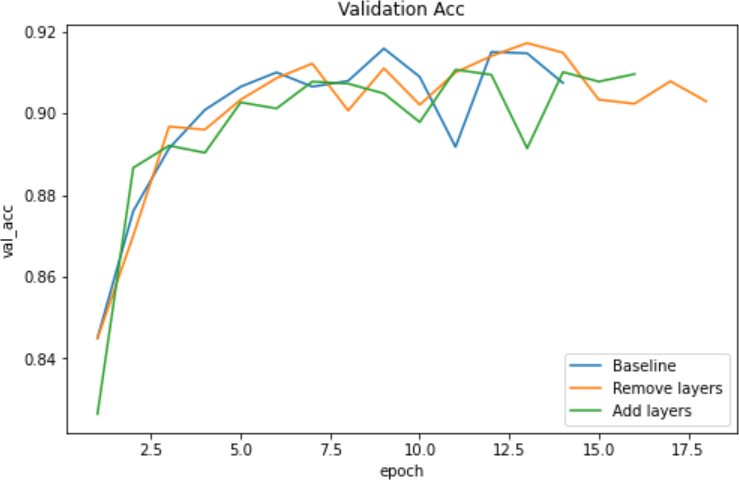
\includegraphics[width=6cm]{./fig/1-cnn-layer.png}%
        }%
        \hspace{1cm}
    \subfloat[\#filters]{%
        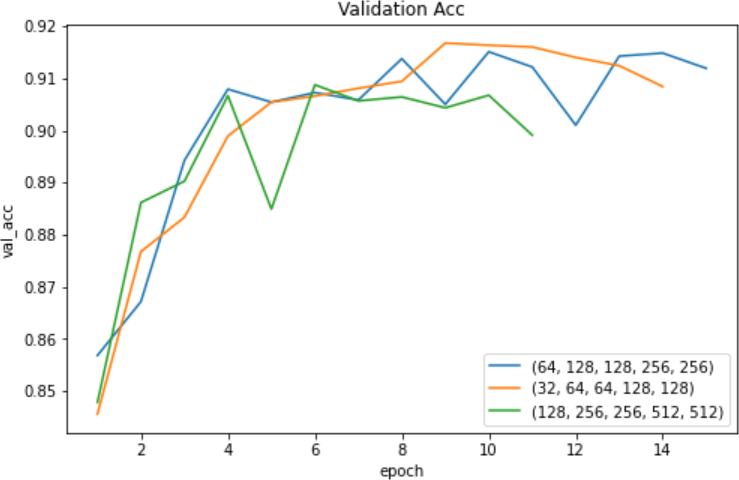
\includegraphics[width=6cm]{./fig/1-cnn-unit.png}%
        }%
        \\
    \subfloat[dropout rate]{%
        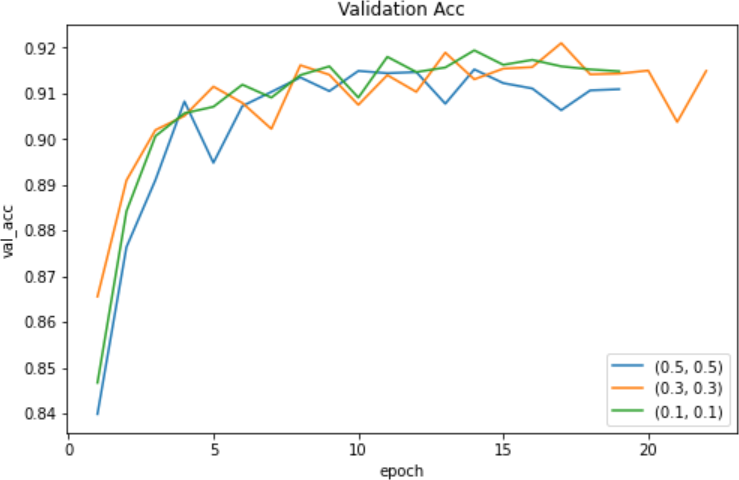
\includegraphics[width=6cm]{./fig/1-cnn-op.png}%
        }%
        \hspace{1cm}
    \subfloat[optimizer]{%
        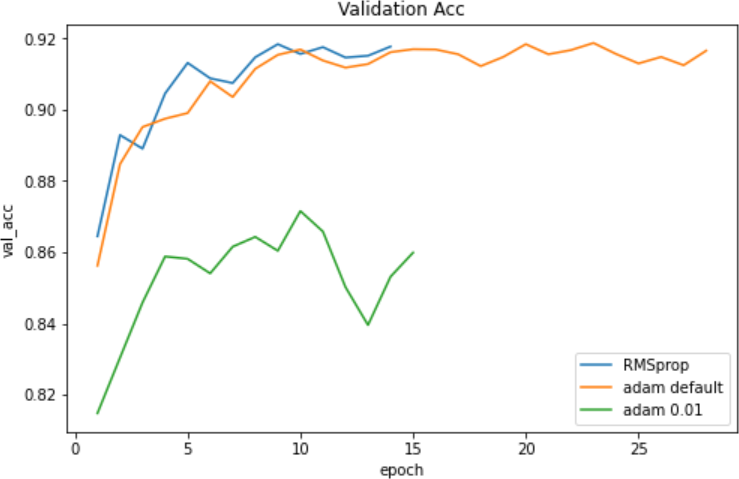
\includegraphics[width=6cm]{./fig/1-cnn-op2.png}%
        }%
    \caption{CNN: Validation Accuracy}
    \label{fig:1-cnn-arch}
\end{figure}
\par
The best model architecture is adding five Conv2D layers with (32, 64, 64, 128, 128) filter setting. Due to the high training cost of CNN, we reduce the parameter space compared to MLP. To be specific, we experiment with different dropout rates and optimizers. Table \ref{tab:1-cnn-hy} and Figure \ref{fig:1-cnn-arch} (c)(d) show the results.
\begin{table}[!ht]
    \centering
    \caption{CNN Hyperparameter Tuning}
    \label{tab:1-cnn-hy}
    \begin{tabular}{llll}
        \toprule
        \textbf{Parameter} & \textbf{Value} & \textbf{Test Loss} & \textbf{Test Accuracy}\\
        \midrule
        dropout rate & 0.1 & 0.3279 & \textbf{0.9183}\\
                     & 0.3 & 0.3613 & 0.9175\\
                     & 0.5 & 0.3713 & 0.9105\\
        \midrule
        optimizer & RMSprop & 0.2768 & 0.9111\\
                  & Adam (learning rate=0.001) & 0.4071 & \textbf{0.9116}\\
                  & Adam (learning rate=0.01) & 0.3658 & 0.8732\\
        \bottomrule
    \end{tabular}
\end{table}
\par 
Table \ref{tab:1-top3-cnn} lists the top three CNN model settings. All settings use the architecture with five Conv2D layers and (32, 64, 64, 128, 128) filter setting.

\begin{table}[!ht]
    \centering
    \caption{Top Three CNN Model Settings}
    \label{tab:1-top3-cnn}
    \begin{tabular}{llll}
        \toprule
        \textbf{Model} & \textbf{dropout rate} & \textbf{optimizer} & \textbf{Test Accuracy}\\
        \midrule
        Top 1 & 0.1 & RMSprop & 0.9183\\
        Top 2 & 0.1 & Adam (learning rate=0.001) & 0.9116\\
        Top 3 & 0.5 & RMSprop & 0.9109\\
        \bottomrule
    \end{tabular}
\end{table}

\subsubsection{CIFAR-10}
We set the models provided in the textbook as baselines for CIFAR-10 data. To test whether performance gains can be translated, we directly use MLP settings in Table \ref{tab:1-top3-mlp} and CNN settings in Table \ref{tab:1-top3-cnn} on CIFAR-10. Besides, we repeat the hyperparameter optimization process to find other possibly better hyperparameter settings. The best MLP new settings are: \{\#layers: 4, \#units: (512, 128, 32, 10), layer activation: relu, kernel initializer: GlorotUniform, kernel regularizer: None, Dropout layers: Yes. rates=(0.1, 0.1, 0.1)\}. And the best CNN new settings are: \{\#Conv2D layers: 5, \#filters: (64, 128, 128, 256, 256), dropout rate: (0.1, 0.1), optimizer: Adam (learning rate=0.001) \}. Table \ref{tab:1-cifar} summarizes the results of our experiments on CIFAR-10.
\begin{table}[!ht]
    \centering
    \caption{CIFAR-10: Performance of Different Settings}
    \label{tab:1-cifar}
    \begin{tabular}{llll}
        \toprule
        \textbf{Category} & \textbf{Model} & \textbf{Test Loss} & \textbf{Test Accuracy}\\
        \midrule
        MLP & Baseline & 1.4616 & 0.4977\\
            & Top 1 in Fashion MNIST & 1.5321 & 0.4559\\
            & Top 2 in Fashion MNIST & 1.4960 & 0.4735\\
            & Top 3 in Fashion MNIST & 1.5921 & 0.4304\\
            & MLP Best New Settings & 1.4300 & \textbf{0.4985}\\
        \midrule
        CNN & Baseline & 1.5516 & 0.6478\\
            & Top 1 in Fashion MNIST & 0.9998 & 0.6969\\
            & Top 2 in Fashion MNIST & 1.0246 & 0.7004\\
            & Top 3 in Fashion MNIST & 0.9959 & 0.6802\\
            & CNN Best New Settings & 1.1895 & \textbf{0.7024}\\
        \bottomrule
    \end{tabular}
\end{table}
\par
According to Table \ref{tab:1-cifar}, the performance gains don't translate to a different dataset.

\subsection{Discussion}
Hyperparameter tuning plays an important role in improving model performance. Deep learning mdoels usually have many hyperparameters. Therefore, we need to use a systematic approach to optimizing hyperparameters. For example, we can apply grid search technique on the parameter space. If the model architecture is very complicated, we may need to use more advanced tuning frameworks, such as Ray Tune, Hyperopt, etc. When exploring the best settings, it is helpful to set callbacks in Keras models to control the training process dynamically. It is worth noting that the best hyperparameter setting on one dataset generally doesn't obtain the best performance on another dataset. That means we should perform hyperparameter tuning on a new dataset even the model structure remains the same.

\section*{Task 2}
\setcounter{section}{2}
\setcounter{subsection}{0}
\subsection{Regression}
The regression model structure is shown in Figure \ref{fig:regression}. And its corresponding results are shown in Table \ref{tab:performance}. Considering this is a regression task, we choose MSE as the loss function and Adam as the optimizer. This model includes 2,207,593 trainable parameters, which is relatively large compared to other models in Task 2. However, the final common sense error is still slightly high, which is 0.7053 hours (about 42.3 minutes). This is mainly caused by the inconsistency between label representation and common sense definition. In other words, representing time in this form disobeys common sense. For example, 11:55 is represented as 11.917, while 0:05 is represented as 0.0833. Even though the difference between 11:55 and 0:05 is only 10 minutes in common sense, their corresponding labels (11.917 and 0.0833) lead to a very high MSE. Therefore, the regression model has a limited final performance.

\begin{figure}[!h]
	\centering
	\begin{minipage}[t]{0.32\textwidth}%并排放两张图片,每张占页面的0.5,下同。
		\centering
		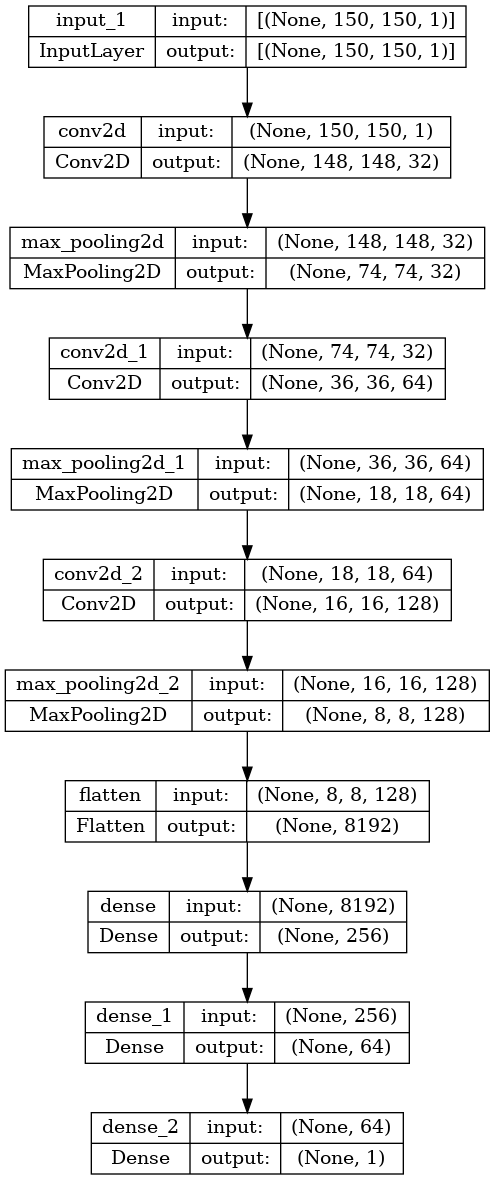
\includegraphics[width=0.8\textwidth, height=7cm]{./fig/reg_model.png}
		\caption{Regression Model}
		\label{fig:regression}
	\end{minipage}
	\begin{minipage}[t]{0.32\textwidth}%并排放两张图片,每张占页面的0.5,下同。
		\centering
		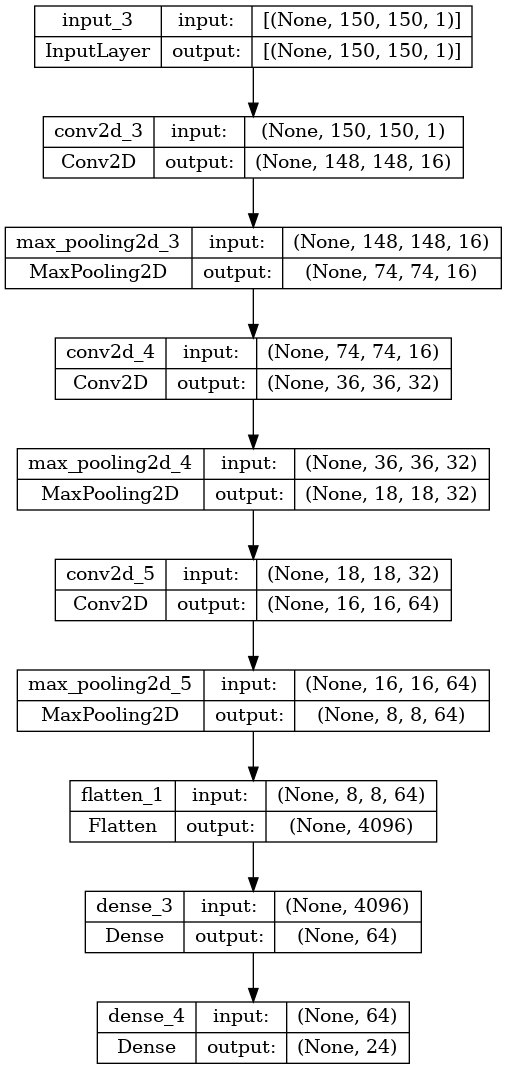
\includegraphics[width=0.8\textwidth, height=7cm]{./fig/class_model.png}
		\caption{Classification Model}
		\label{fig:classification}
	\end{minipage}
	\begin{minipage}[t]{0.32\textwidth}%并排放两张图片,每张占页面的0.5,下同。
		\centering
		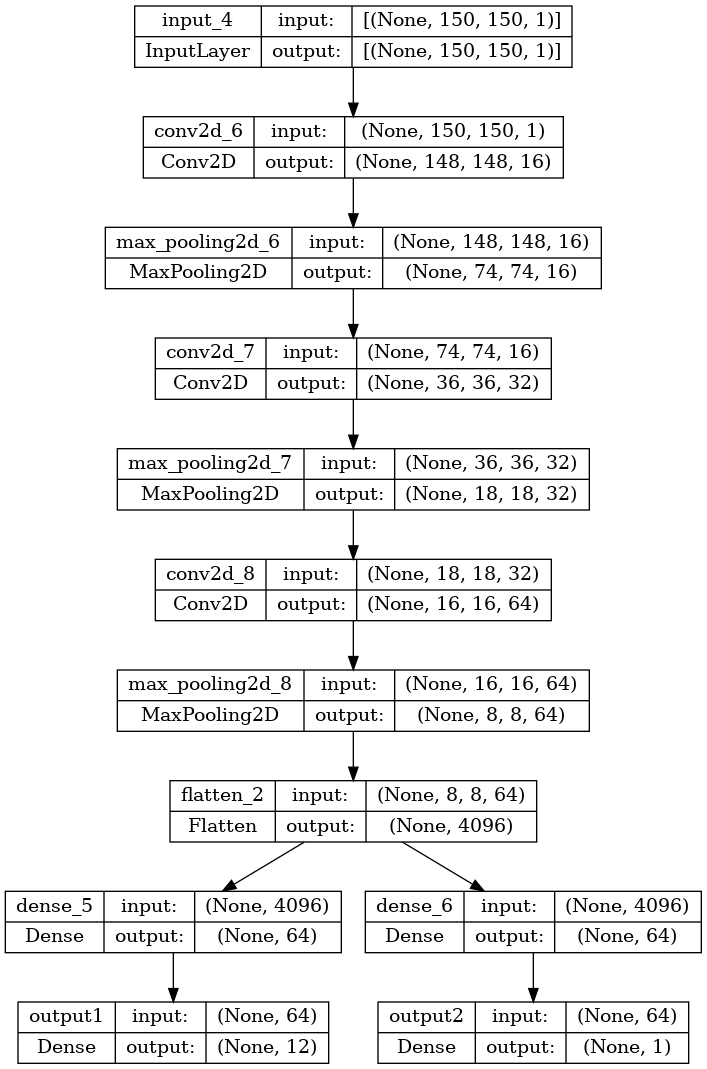
\includegraphics[width=\textwidth, height=7cm]{./fig/multi_model.png}
		\caption{Multi-head Model}
		\label{fig:multi-head}
	\end{minipage}
\end{figure}
    \begin{table}[!ht]
	\caption{Results and Algorithm Comparison}
	\label{tab:performance}
	\centering
	\begin{tabular}{ll}
		\toprule
		\textbf{Model} & \textbf{Common Sense Error (hours)} \\
		\midrule
		Regression & 0.7053 \\
		Classification (24 classes) & 0.6206 \\
		Classification (72 classes) & 0.9517 \\
		Classification (720 classes) & 3.0309 \\
		Multi-head model& 0.6161 \\
		Label transformation & 0.3447 \\
        Label transformation (fine-tuned) & \textbf{0.1921} \\
		\bottomrule
	\end{tabular}
\end{table}

\subsection{Classification}
Figure \ref{fig:classification} illustrates the architecture of classification model. Table \ref{tab:performance} reports the corresponding results. We experiment with 24, 72, and 720 classes in the classification task, where models are only different in the last output layer. We use the cross entropy loss function and the Adam optimizer, which are the common choices for multi-class classification task. Although the classification model has much fewer trainable parameters (287,064 trainable parameters for 24 classes), the performance of 24 classes model achieves 0.6206 hours (about 37.2 minutes), which is better than the regression model. However, the increase of the categories impairs model performance. In the case of 720 classes, the model even doesn't converge and has a very high common sense error. The reason is that using time intervals as class labels has many drawbacks. The first problem is that this kind of label representation can't measure the degree of difference between two categories. For example, 0:01 and 0:31 belong to different categories in 24 classes model. Meanwhile, 0:01 and 6:00 are also in different categories. Although the common sense error between 0:01 and 6:00 is much larger than that between 0:01 and 0:31, the cross entropy loss function treats the two cases as the same. The second problem is that the trade-off between the length of sampling interval and the number of samples is hard to be determined. If we group the samples into fewer classes, each class will cover a longer time interval and therefore have more samples. Then, the model will be well trained because there are sufficient samples in each class. Nonetheless, the common sense error of each class will become rather high. We still use the model with 24 classes as an example. In this model, 0:01 and 0:29 are classified into the same class even they are almost half an hour apart, which causes the major deviation from the common sense. On the contrary, if we classify the samples into more classes whose corresponding time interval is shorter, the common sense error within each class will decrease. However, the model itself will be underfitting due to the deficiency of samples for each class. Considering the case of constructing model for 720 classes, the average number of samples for each class is only 25, which is generally insufficient for training CNN.

\subsection{Multi-head Model}
We display the model structure and corresponding results of multi-head model in Figure \ref{fig:multi-head} and Table \ref{tab:performance}. We build the model with two heads --- one for predicting hours and the other for predicting minutes. And we regard two-head outputs as the multi-class classification task and the regression task, respectively. For classification task of predicting hours, we consider 12 hours as 12 different categories and use cross entropy as the loss function. For regression task of predicting minutes, we select MSE as the loss function. This model contains 548,557 trainable parameters. Its common sense error finally achieves 0.6161 hours (about 37.0 minutes), which is the best result up to now. The reason of improvement is that using the multi-head model can utilize characteristics of different aspects of target labels. To be specific, considering the hour prediction as a classification task will only lead to a model with 12 classes, which means the number of samples in each class is adequate for training. Meanwhile, it is reasonable to model the minute forecast as a regression task, since the target values distribute in a wide range $\{0,\dots,59\}$. The flexibility of the multi-head model enables us to combine these two tasks and obtain the predictions of hours and minutes simultaneously, which helps to improve the model performance. We would like to highlight one point. That is we should normalize the minute lables for regression head to the interval [0,1) by dividing them by 60. Otherwise, the disproportion between the cross entropy loss for hours and the MSE loss for minutes will have a negative impact on model training. It is worth noting that the deficiencies of label representations are still not overcome in the multi-head model, despite the performance improvement obtained. Therefore, we will use label transformation to enhance the model performance further in the next section.

\subsection{Label Transformation}
Based on the experience of previous tasks, we find that directly setting the value of hours and minutes as targets fails to conform to the common sense. And the inconformity is the main cause of large common sense errors. Inspired by the periodic functions, we use sine and cosine functions to represent angles on the unit circle to resolve the inconsistency.

We assume the ray that starts at the center of the clock and passes through the zero o'clock as the polar axis. It is obvious that the angle $\theta$ between the hour hand and the axis contains all of the information about time. Then, we apply the sine function on angle $\theta$. We still use the previous example, 0:05 and 11:55, to show the difference. Computing the angle $\theta$ for 0:05 as well as 11:55 is straightforward, where results are 0.0436 rads and 6.240 rads. As we can see, $\sin(0.0436)$ and $\cos(6.240)$ equal to 0.0436 and -0.0436 respectively, which are very close to each other due to the property of periodic functions. That is exactly what we want for our labels.

But there is another problem. The sine function maps different angles between the hour hand and the axis to the same value even if they represent different time. For example, 1:00 ($\frac{\pi}{6}$) and 5:00 ($\frac{5\pi}{6}$) are both projected to 0.5. Fortunately, we can apply the cosine function to distinguish these angles. Above all, we need to transform the original label [hour, minute] to [$\sin(\theta)$, $\cos(\theta)$]. Therefore, the number of nodes in output layer should be two --- one for sine and the other for cosine. The sine function and cosine function both have the range of $[-1,1]$. And we know that tanh activation function also has the same range. Thus, applying the tanh activation function in the output layer is perfect. And we consider it as a regression problem as well. Figure \ref{fig:labeltrans} shows the model architecture.

\begin{figure}[!h]
	\centering
	\begin{minipage}[t]{0.4\textwidth}%并排放两张图片,每张占页面的0.5,下同。
		\centering
		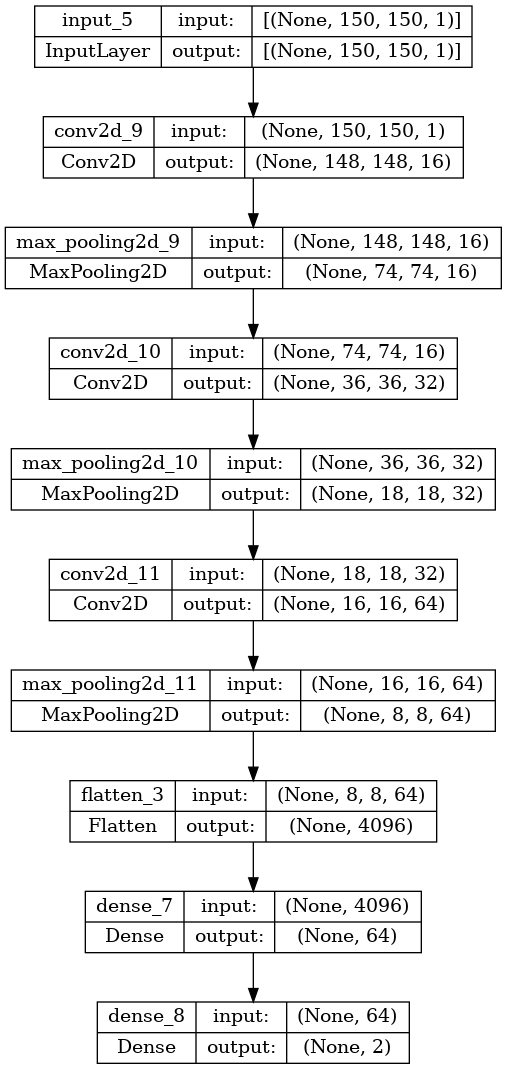
\includegraphics[width=0.7\textwidth, height=7cm]{./fig/label_model.png}
		\caption{Label Transformation Model}
		\label{fig:labeltrans}
	\end{minipage}
    \hspace{0.8cm}
	\begin{minipage}[t]{0.4\textwidth}%并排放两张图片,每张占页面的0.5,下同。
		\centering
		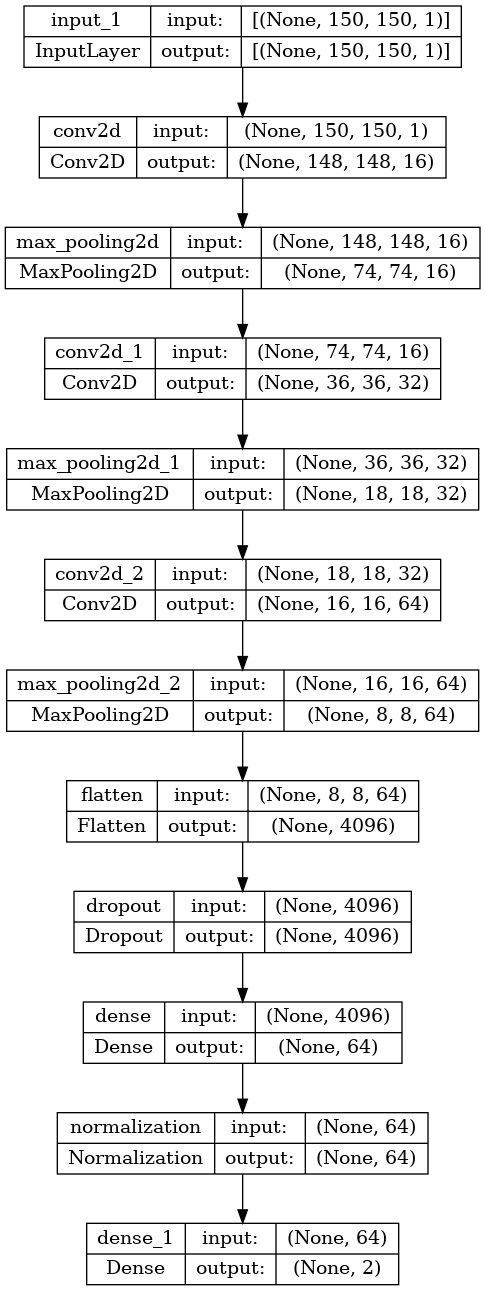
\includegraphics[width=0.6\textwidth, height=7cm]{./fig/final_model.png}
		\caption{Final Model}
		\label{fig:final}
	\end{minipage}
\end{figure}

The regression model with label transformation works well. Its performance is shown in Table \ref{tab:performance}. It only has 285,634 trainable parameters but achieves 0.3447 hours (about 20.7 minutes) in common sense error, which is the best result up to now. In the next section, we will fine-tune this model using the knowledge gained from previous tasks and obtain our final model for Task 2.

\subsection{Final Model}
The structure and performance of our final model are shown in Figure \ref{fig:final} and Table \ref{tab:performance}. Compared to the model in Section 2.4, we make several adjustments. Firstly, we use LeakyReLu instead of ReLu as the activation function in all hidden layers to avoid the vanishing gradient problem. In addition, we apply L2 regularization in each layer which contains trainable parameters to alleviate overfitting. Besides, a Dropout layer is added after the Flatten layer, and a Normalization layer is applied after the first Dense layer. Finally, we use the combination of checkpoints and early stopping as in Task 1 and set the learning rate to a small value.

Our final model achieves 0.1921 hours (about 11.5 minutes) in common sense error, which outperforms all the other models, especially the first three models. Periodic functions, sine and cosine, successfully coordinate the time labels following the common sense, which contributes to the major improvement. In conclusion, a well-designed label is essential to training and evaluating neural networks. After determining a suitable model structure, fine-tuning process can as well enhance the model performance further.

\section*{Task 3}
\setcounter{section}{3}
\setcounter{subsection}{0}
\subsection{Datasets}
We use two datasets in Task 3. Firstly, we explore the performance of different model architectures and the effects of different parameter settings with MNIST data. After that, we leverage the power of generative models on Butterfly \& Moth data. \par
We directly call Tensorflow API to download the MNIST dataset. However, the original dataset is also available on \url{https://deepai.org/dataset/mnist}. MNIST dataset contains 70,000 grayscale images (28 $\times$ 28 $\times$ 1), whose content is handwritten numbers. \par
Butterfly \& Moth is an open source dataset on Kaggle. There are 13,639 RGB images (224 $\times$ 224 $\times$ 3) composed of 100 butterfly or moth species. Link of the dataset is \url{https://www.kaggle.com/datasets/gpiosenka/butterfly-images40-species?resource=download}.

\subsection{Experimental Set-up}
All experiments are deployed on two servers. Server 1 has an Intel(R) Xeon(R) Platinum 8358P CPU and a RTX A5000 GPU, while server 2 has an Intel(R) Xeon(R) E5-2680 v4 CPU and a TITAN Xp GPU. Table \ref{tab:3-hyper} summarizes the hyperparameter values in the experiments. The following describes the process of our experiments.
\begin{table}[!ht]
    \centering
    \caption{Hyperparameter Settings}
    \label{tab:3-hyper}
    \begin{tabular}{lll}
        \toprule
        \textbf{Parameter} & \textbf{Value} & \textbf{Meaning}\\
        \midrule
        cae\_latent\_dim & 32 & Dimensions of the latent space in CAEs.\\
        cae\_epoch & 10 & The number of training epochs in CAEs.\\
        vae\_latent\_dim & 32 & Dimensions of the latent space in VAEs.\\
        vae\_epoch & 20 (MNIST) / 100 (Butterfly \& Moth) & The number of training epochs in VAEs.\\
        gan\_latent\_dim & 256 & Dimensions of the latent space in GANs.\\
        gan\_epoch & 20 (MNIST) / 250 (Butterfly \& Moth) & The number of training epochs in GANs.\\
        \bottomrule
    \end{tabular}
\end{table}

\subsubsection{MNIST}
We modify the model architecture to decrease the model complexity and match the data better. Specially, we build the basic convolutional network with four Conv2D layers and construct the basic deconvolutional network with one Conv2DTranspose layer. Figure \ref{fig:3-model} illustrates our model settings. There is no need to resize the images due to the modification of the model.
\begin{figure}[!ht]
    \centering
    \subfloat[Convolutional network]{%
        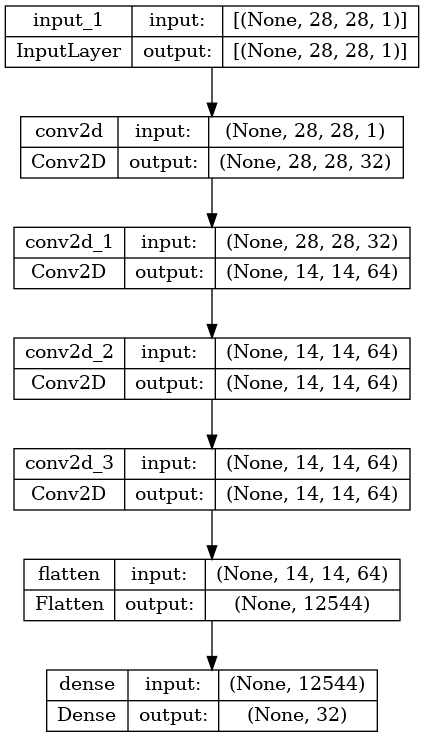
\includegraphics[height=4cm, width=4cm]{./fig/conv.png}%
        \label{fig:conv}%
        }%
        \hspace{1.5cm}
    \subfloat[Deconvolutional network]{%
        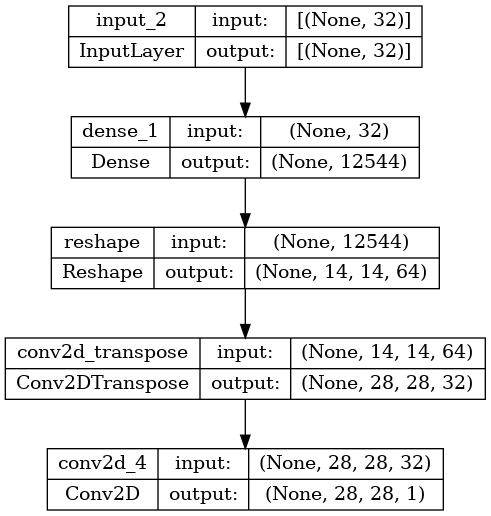
\includegraphics[height=4cm, width=5cm]{./fig/deconv.png}%
        \label{fig:deconv}%
        }%
    \caption{Model Structure}
    \label{fig:3-model}
\end{figure}

\subsubsection{Butterfly \& Moth}
We rescale the images to 64 $\times$ 64 $\times$ 3 and directly apply the model architecture provided in the notebook when working with Butterfly \& Moth data.

\subsection{Results}
\textbf{CAEs}. Figure \ref{fig:3-cae} shows the reconstructed images from CAEs. It is easy to see that CAEs have captured the main features in the original images.
\begin{figure}[!ht]
    \centering
    \subfloat[MNIST: Original Images]{
        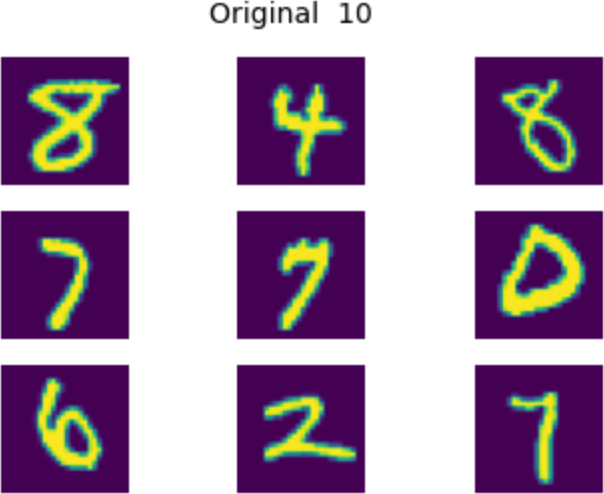
\includegraphics[width=5.6cm]{./fig/mnist-cae-ori.png}
    }
    \hspace{1cm}
    \subfloat[MNIST: Reconstructed Images]{
        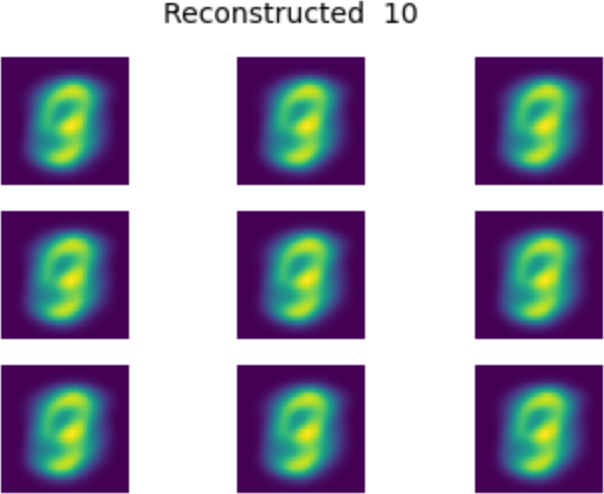
\includegraphics[width=5.6cm]{./fig/mnist-cae-re.png}
    }
    \\
    \subfloat[Butterfly \& Moth: Original Images]{
        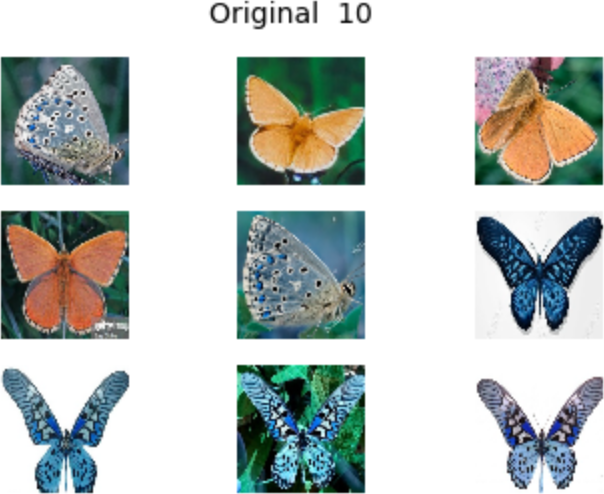
\includegraphics[width=5.6cm]{./fig/bm-cae-ori.png}
    }
    \hspace{1cm}
    \subfloat[Butterfly \& Moth: Reconstructed Images]{
        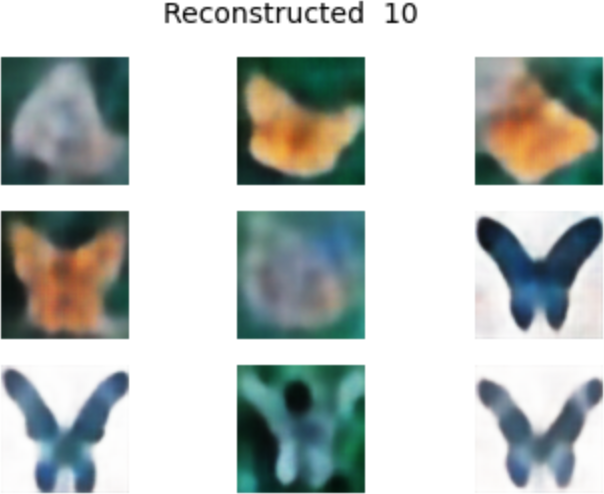
\includegraphics[width=5.6cm]{./fig/bm-cae-re.png}
    }
    \caption{Results of CAEs}
    \label{fig:3-cae}
\end{figure}
\par~\\
\textbf{VAEs}. We explore the learned latent space with linear interpolation technique. Firstly, we sample a point from the latenty space by generating its coordinates from a standard normal distribution. Then, we change one or two coordinates along the straight line in the latent space, while keep other coordinates unchanged. For MNIST dataset, we apply linear interpolation on the 10th and 27th coordinates simultaneously, which are related to the shape of the number. Figure \ref{fig:vae-mnist} shows the visualization results.
\begin{figure}[!ht]
    \centering
    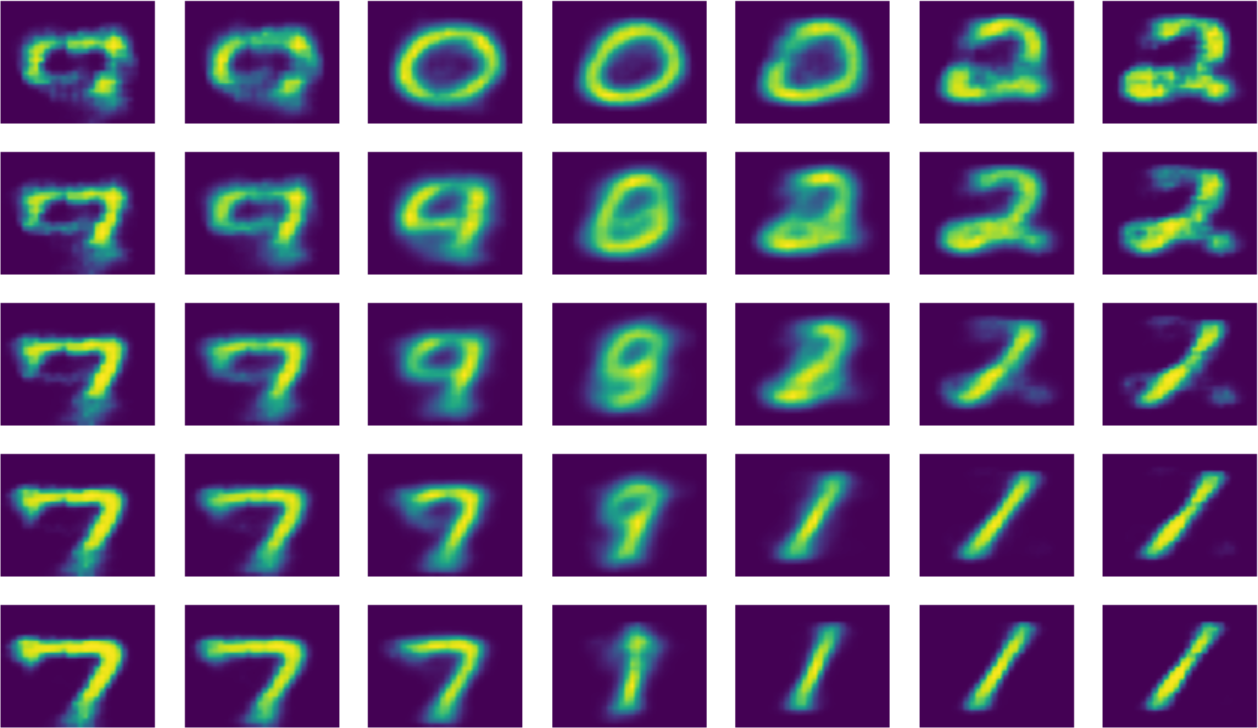
\includegraphics[width=10cm, height=5cm]{./fig/mnist-vae.png}
    \caption{VAEs: MNIST Data}
    \label{fig:vae-mnist}
\end{figure}
As for Butterfly \& Moth data, we linearly interpolate the 6th and 29th coordinates, whose outputs are presented in Figure \ref{fig:vae-bm}. According to Figure \ref{fig:vae-bm}, the 6th coordinate is related to the color of wings, while the 29th coordinate is concerned with the width of wings.
\begin{figure}[!ht]
    \centering
    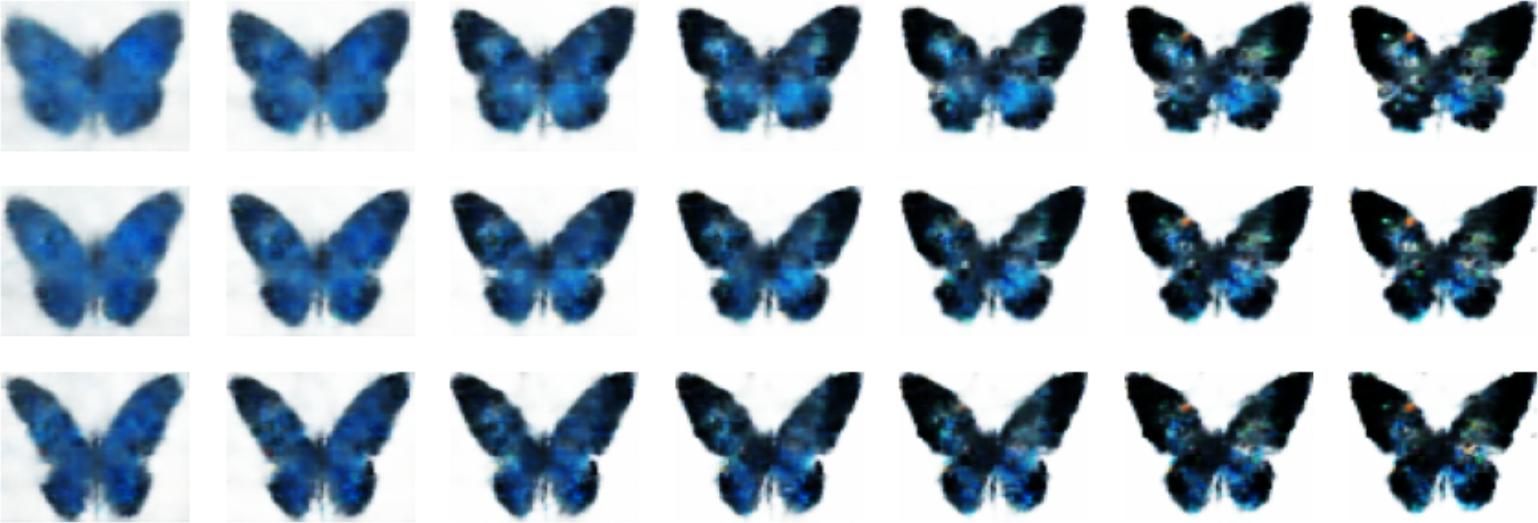
\includegraphics[width=10cm, height=4cm]{./fig/bm-vae.png}
    \caption{VAEs: Butterfly \& Moth Data}
    \label{fig:vae-bm}
\end{figure}
\par~\\
\textbf{GANs}. We visualize the outputs of linear interpolation in the same way as VAEs. We change the 1st, 120th, and 126th coordinates for MNIST data to obtain different numbers. Figure \ref{fig:gan-mnist} shows the generated images. For Butterfly \& Moth data, we change the 40th coordinate, which is related to the color and the posture of the butterfly. Figure \ref{fig:gan-bm} shows the generated butterfly.
\begin{figure}[!ht]
    \centering
    
\includegraphics[width=10cm, height=1cm]{./fig/gan-1.png}
    
\includegraphics[width=10cm, height=1cm]{./fig/gan-2.png}
    
\includegraphics[width=10cm, height=1cm]{./fig/gan-3.png}
    \caption{GANs: MNIST Data}
    \label{fig:gan-mnist}
\end{figure}
\begin{figure}[!ht]
    \centering
    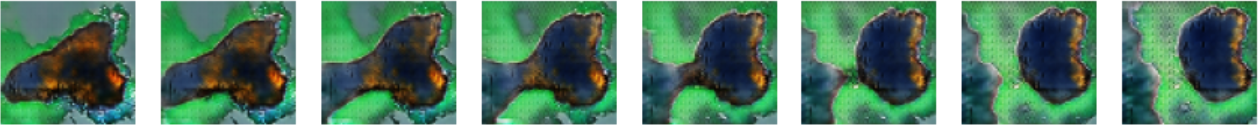
\includegraphics[width=10cm, height=1cm]{./fig/gan-bm.png}
    \caption{GANs: Butterfly \& Moth Data}
    \label{fig:gan-bm}
\end{figure}

\subsection{Discussion: Model Comparison}
CAEs are autoencoders that apply the CNN architecture to compress the input images into a lower dimensional latent space and reconstruct the images from the learned latent space. Using an encoder/decoder structure enables CAEs to capture as much information about data as possible, even without labels. However, CAEs are deterministic. That means there is a one-to-one relationship between the input and output in CAEs. Therefore, CAEs can't generate new samples. Based on the architecture of the traditional autoencoder, VAEs introduce randomness into the model by assuming a prior distribution of latent space and infering the posterior distribution during the training process. In most cases, we choose the standard Gaussian distribution as prior distribution, which helps the latent space to be complete and continuous. The probabilistic nature allows VAEs to generate new images from random noise.\par
GANs are designed for generating new samples. Instead of inferring the distribution of latent space, GANs sample from random noise and learn a transformation to imitate the real distribution of data. Gans improve the quality of imitations by training a discriminator to distinguish between generated samples and real samples.\par
In summary, VAEs sample from a prior distribution and infer the real distribution of latent space, while GANs sample from random noise and learn the data transformation by encouraging the competition between generator and discriminator.

\section*{Contributions}
\begin{tabular}{ll}
    \textbf{Name} & \textbf{Contribution}\\
    Chenyu Shi & Task 1 code, Task 2 code, Task 2 report.\\
    Shupei Li & Task 1 code, Task 1 report, Task2 code, Task 3 code, Task 3 report.\\
    Shuang Fan & Task 1 code, Task 1 report.\\
\end{tabular}
\end{document}
